% !TEX program = lualatex
%==============================================================================
%  Directional Partial-Wave Sweeps and the Krylov Solve.
%  The propagator matvec for elastic multiple scattering on a depth-stratified
%  voxel grid.
%
%  Self-contained LuaLaTeX source. Compile with:
%      latexmk -lualatex DirectionalSweepSolver.tex
%==============================================================================
\documentclass[11pt,a4paper]{article}

% --- LuaLaTeX font handling -------------------------------------------------
\usepackage{fontspec}
\setmainfont{Latin Modern Roman}

% --- Mathematics ------------------------------------------------------------
\usepackage{amsmath}
\usepackage{amssymb}
\usepackage{mathtools}

% --- Layout and typography --------------------------------------------------
\usepackage[margin=1in]{geometry}
\usepackage{microtype}
\usepackage{xcolor}
\usepackage{booktabs}

% --- Graphics ---------------------------------------------------------------
\usepackage{tikz}
\usetikzlibrary{arrows.meta}

% --- Hyperlinks -------------------------------------------------------------
\usepackage[colorlinks=true,
            linkcolor=blue!55!black,
            citecolor=blue!55!black,
            urlcolor=blue!55!black]{hyperref}
\hypersetup{
  pdftitle={Directional Partial-Wave Sweeps and the Krylov Solve},
  pdfauthor={Tod Nestor}
}

% --- Macros -----------------------------------------------------------------
\newcommand{\ii}{\mathrm{i}}
\newcommand{\rd}{\mathrm{d}}
\newcommand{\Tz}{T_0}
\newcommand{\Gz}{G_0}
\newcommand{\kpar}{\mathbf{k}_{\parallel}}

\title{\bfseries Directional Partial-Wave Sweeps and the Krylov Solve\\[4pt]
\large The propagator matvec for elastic multiple scattering on a
depth-stratified voxel grid}
\author{Tod Nestor}
\date{16 June 2026}

\begin{document}
\maketitle

\begin{abstract}
The multiple scattering of elastic waves by voxels superimposed on a depth-stratified
background is a Foldy--Lax / volume integral equation, $T=\Tz(I-\Gz\Tz)^{-1}$, solved by a
Krylov method whose only nontrivial operation is the application of the background propagator
$\Gz$. This note describes that application as an alternating-direction partial-wave summation:
the lateral coupling is summed by constant-$z$ left-right ($k_x$) and constant-$(z,x)$ in-out
($k_y$) cumulative-phase sweeps, and the coupling between depth planes by the up-down Kennett
reflectivity recursion ($k_z$). Choosing the lateral directions for the in-plane coupling sums
the propagator along axes in which the voxels are separated, so the $k_z$ partial-wave sum that
diverges at zero depth separation is never evaluated. The sweeps are a pure forward matvec; all
multiple scattering, to every order, is resolved by the Krylov iterations.
\end{abstract}

\bigskip
\noindent\textbf{Companion series.}\enspace{\small\itshape One of a companion series on elastic
multiple scattering from cubic heterogeneities on a depth-stratified background, the T-matrix
programme $T=T_0(I-G_0T_0)^{-1}$: \textbf{(I)}~the stratified inter-site propagator, the
same-depth convergence theory, the SH and P/SV traction kernels, interplane side scattering and
the first-shell near stencil (\texttt{EwaldIntraPlanePropagator}); \textbf{(II)}~the
contrast-source volume integral equation and the CG-FFT / seismic grid T-matrix lineage
(\texttt{ContrastSourceVIE}); \textbf{(III)}~the directional partial-wave sweep matvec and the
Krylov multiple-scattering solve (\texttt{DirectionalSweepSolver}); with the empirical companion
\texttt{RQ1\_Planar\_Decomposition\_Proposal}. This is note~(III).}

\tableofcontents
\bigskip

%==============================================================================
\section{The system, and where the cost lives}
%==============================================================================

Voxels (cubic cells) are superimposed on a background that carries the lateral average of the
medium at each depth: laterally homogeneous within a constant-$z$ plane, layered in $z$. Each
voxel has an on-site T-matrix $\Tz$, the single-cell scatterer (Eshelby with the $r=0$
delta-function correction up to the 27-component Galerkin form, the self-term already closed),
and the voxels are coupled by the background propagator $\Gz$. The multiple scattering is the
Foldy--Lax system \cite{Foldy1945,Lax1951,GubernatisDomanyKrumhansl1977}
\begin{equation}
\label{eq:foldylax}
(I-\Gz\Tz)\,\psi=\psi^{\mathrm{inc}},\qquad T=\Tz\,(I-\Gz\Tz)^{-1},
\end{equation}
where $\psi$ collects the exciting (incoming) fields at the voxels. The operator $\Tz$ is
block-diagonal and local. The whole cost is the off-diagonal $\Gz$: the inter-voxel
communication. The strategy is to solve \eqref{eq:foldylax} by a Krylov method whose
matrix-vector product is one application of $\Gz$, and to make that application fast.

The essential point is the division of labour. The application of $\Gz$ is a \emph{forward}
operation, a summation of partial waves that carries the radiation of every voxel to every
other. It contains no inversion and no embedding. All of the multiple scattering, the
reverberations to every order, is built and resummed by the Krylov iterations, not by the
propagator.

%==============================================================================
\section{The matvec is a partial-wave summation}
%==============================================================================

Given source amplitudes $b=\Tz\psi$ at the voxels, the matvec returns the field they radiate,
$\psi'=\Gz\,b$. For the homogeneous part of the background the propagator is a sum of partial
waves, and a partial wave's phase accumulates linearly in space: $e^{\ii k x}$ at the next
voxel is the current one times $e^{\ii k p}$, with $p$ the pitch. The sum is therefore built by
carrying that running phase along a line, one term added per voxel. This is the sweep. The only
freedom is which axis to sum along, and the choice is dictated by where the voxels are
separated.

\begin{figure}[h]
\centering
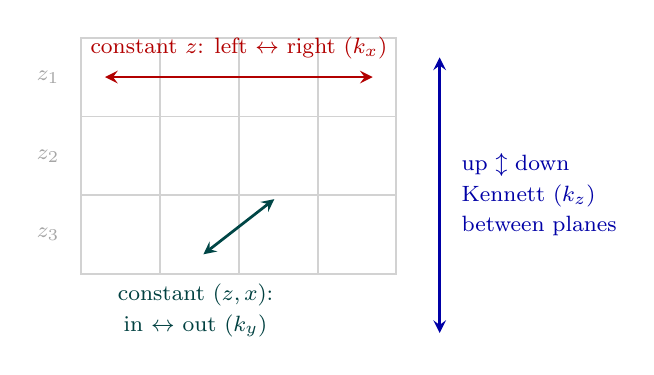
\begin{tikzpicture}[>=stealth, line width=0.7pt]
  \foreach \r in {0,1,2}{
    \foreach \c in {0,1,2,3}{ \draw[gray!35] (\c,-\r) rectangle (\c+1,-\r+1); }
  }
  \node[gray!70, anchor=east] at (-0.15,0.5) {\footnotesize $z_1$};
  \node[gray!70, anchor=east] at (-0.15,-0.5) {\footnotesize $z_2$};
  \node[gray!70, anchor=east] at (-0.15,-1.5) {\footnotesize $z_3$};
  % left-right (k_x) on top row
  \draw[<->, red!70!black, line width=1pt] (0.3,0.5)--(3.7,0.5);
  \node[red!70!black, anchor=south] at (2,0.6)
        {\footnotesize constant $z$: left $\leftrightarrow$ right ($k_x$)};
  % up-down Kennett (k_z)
  \draw[<->, blue!65!black, line width=1pt] (4.55,0.75)--(4.55,-2.75);
  \node[blue!65!black, anchor=west, align=left] at (4.7,-1.0)
        {\footnotesize up $\updownarrow$ down\\[-1pt]\footnotesize Kennett ($k_z$)\\[-1pt]\footnotesize between planes};
  % in-out (k_y) perspective at a voxel
  \draw[<->, teal!55!black, line width=1pt] (1.55,-1.75)--(2.45,-1.05);
  \node[teal!50!black, anchor=north, align=center] at (1.45,-2.0)
        {\footnotesize constant $(z,x)$:\\[-1pt]\footnotesize in $\leftrightarrow$ out ($k_y$)};
\end{tikzpicture}
\caption{The $\Gz$ matvec as three directional partial-wave sweeps over the voxel grid
(cross-section; the third axis $y$ runs into the page). Within each depth plane the lateral
coupling is summed by constant-$z$ left-right ($k_x$) and constant-$(z,x)$ in-out ($k_y$)
cumulative-phase sweeps; the coupling between depth planes is the up-down Kennett reflectivity
recursion ($k_z$). The lateral directions carry the in-plane coupling along axes of nonzero
separation, so the $k_z$ sum is never evaluated at $\Delta z=0$.}
\label{fig:sweeps}
\end{figure}

\subsection{Lateral sweeps: constant-$z$ left-right and constant-$(z,x)$ in-out}
\label{sec:lateral}

Within a depth plane the background is homogeneous, so the lateral propagation is pure phase,
with no background reflections to sum. Split the in-plane propagator on the $k_x$ pole into a
right-going and a left-going partial wave and sum each by a sweep in its own direction. With
$a^+$ the right-going accumulated field, $s_n$ the source radiated at voxel $n$, and
$\Phi_x=e^{\ii k_x p}$ the one-pitch lateral propagator,
\begin{equation}
\label{eq:sweep}
a^+_{n+1}=\big(a^+_n+s_n\big)\,\Phi_x \quad(\text{left to right}),
\qquad
a^-_{n-1}=\big(a^-_n+s_n\big)\,\Phi_x \quad(\text{right to left}).
\end{equation}
Each partial wave is carried along the direction in which it decays: the right-going evanescent
branch $e^{-\kappa_{x\perp}x}$ is swept to the right, the left-going branch to the left, so the
growing exponential is never formed and no reflection/transmission bookkeeping is needed for
stability. The in-out sweep in $y$ is identical, run along each constant-$(z,x)$ line on the
$k_y$ pole. The two together sum the full in-plane partial-wave series as nested
one-dimensional phase accumulations.

\subsection{Vertical sweep: up-down Kennett between depth planes}

In $z$ the background is not homogeneous: the lateral average changes from plane to plane, so
the depth-average layering has its own reflections and transmissions. The coupling between
depth planes is therefore the up-down Kennett reflectivity recursion \cite{Kennett1983} on the
$k_z$ pole, propagating the source amplitudes through the layered background and summing its
internal up/down multiples. This is the one sweep that carries reflection and transmission
coefficients, and it does so for the \emph{background} layering, not for the heterogeneity; it
is the standard invariant-embedding recursion, stable by construction, and its coefficients
depend only on the background and are formed once. The heterogeneity scattering remains entirely
in $\Tz$ and the Krylov loop.

\subsection{Why these directions}
\label{sec:why}

The conventional construction sums the in-plane coupling on the $k_z$ pole, the up/down
decomposition, whose surviving $(k_x,k_y)$ integral loses its convergence factor
$e^{-\kappa_\perp|\Delta z|}$ at $\Delta z=0$ and diverges at equal depth. The lateral split
avoids it outright: the in-plane coupling is summed on the $k_x$ and $k_y$ poles, along which
distinct in-plane voxels are separated, so the divergent same-depth $k_z$ sum is never the one
evaluated. The $k_z$ sweep is used only between planes, where $\Delta z\neq 0$ and the Kennett
recursion is exact and stable. Every sweep marches along an axis of nonzero separation.

\subsection{The same-depth term in a stratified background}
\label{sec:intraplane}

The lateral sweep of \S\ref{sec:lateral} sums the same-depth coupling of the \emph{whole space}.
That is not the whole of it. When the background is stratified, two voxels at the same depth are
also coupled by paths that leave one voxel, reflect from a layer boundary above or below, and
return to the plane. Those paths are absent from the lateral sweep by construction, because the
$k_x$ residue carries only the direct term.

They cannot simply be added by evaluating the stratified propagator at $\Delta z=0$ and
integrating: that is the divergence of \S\ref{sec:why}, and it is present in the stratified
kernel exactly as in the whole-space one, its strain--strain block growing like $|k_x|$. The
resolution is to subtract it. Writing $\Gz^{\mathrm{lay}}$ for the stratified propagator between
a plane and itself and $\Gz^{\infty}$ for the whole-space kernel at equal depth,
\begin{equation}
\label{eq:intrasplit}
\Gz^{\mathrm{lay}}(\Delta z = 0) \;=\; \underbrace{\Gz^{\infty}(\Delta z = 0)}_{\text{lateral sweep, by }k_x\text{ residue}}
\;+\; \underbrace{\Delta\Gz}_{\text{reverberation only}} ,
\end{equation}
and the two terms on the right are individually non-integrable while their difference is not.
Every path contributing to $\Delta\Gz$ travels at least twice the distance $H$ to the nearest
interface, so it carries $e^{\ii k_z 2H}$ and $\Delta\Gz$ decays exponentially in $k_x$. Its
$k_x$ integral therefore converges, and the divergence cancels between the two terms rather than
being regularised in either.

\begin{figure}[h]
\centering
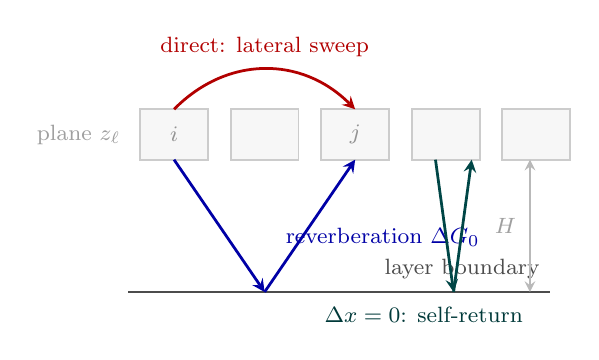
\begin{tikzpicture}[>=stealth, line width=0.7pt]
  % --- the depth plane of voxels ---
  \foreach \c in {0,1,2,3,4}{
    \draw[gray!40, fill=gray!6] (\c*1.15,-0.32) rectangle ++(0.86,0.64);
  }
  \node[gray!75, anchor=east, font=\footnotesize] at (-0.12,0) {plane $z_\ell$};
  \node[font=\footnotesize, gray!85] at (0.43,0)  {$i$};
  \node[font=\footnotesize, gray!85] at (2.73,0)  {$j$};

  % --- layer boundary below ---
  \draw[black!70, line width=1pt] (-0.15,-2.0) -- (5.2,-2.0);
  \node[black!70, anchor=south east, font=\footnotesize] at (5.2,-1.96)
       {layer boundary};
  \draw[<->, gray!55] (4.95,-0.32) -- (4.95,-2.0);
  \node[gray!75, font=\footnotesize, anchor=east] at (4.9,-1.16) {$H$};

  % --- DIRECT term: in-plane, summed by the k_x residue ---
  \draw[->, red!70!black, line width=1pt]
       (0.43,0.32) .. controls (1.1,1.0) and (2.05,1.0) .. (2.73,0.32);
  \node[red!70!black, anchor=south, font=\footnotesize] at (1.58,0.86)
       {direct: lateral sweep};

  % --- REVERBERATION: down to the boundary and back up to the same plane ---
  \draw[->, blue!65!black, line width=1pt] (0.43,-0.32) -- (1.58,-2.0);
  \draw[->, blue!65!black, line width=1pt] (1.58,-2.0) -- (2.73,-0.32);
  \node[blue!65!black, font=\footnotesize, anchor=west] at (1.72,-1.3)
       {reverberation $\Delta\Gz$};

  % --- SELF-RETURN: the Delta x = 0 entry ---
  \draw[->, teal!55!black, line width=1pt] (3.75,-0.32) -- (3.98,-2.0);
  \draw[->, teal!55!black, line width=1pt] (3.98,-2.0) -- (4.21,-0.32);
  \node[teal!45!black, font=\footnotesize, anchor=north] at (3.6,-2.06)
       {$\Delta x=0$: self-return};
\end{tikzpicture}
\caption{The same-depth interactions of \eqref{eq:intrasplit}, at one depth plane. The
\textcolor{red!70!black}{direct} whole-space coupling between voxels $i$ and $j$ is summed by the
lateral sweep, on the $k_x$ pole, exactly. The \textcolor{blue!65!black}{reverberation} leaves the
plane, reflects from a layer boundary a distance $H$ away and returns to it; the lateral sweep
cannot carry it, and it is what $\Delta\Gz$ supplies. Both terms diverge on their own --- each
grows like $|k_x|$ --- and their difference does not, because every reverberating path travels at
least $2H$ and so carries $e^{\ii k_z 2H}$. The \textcolor{teal!55!black}{third path} is the same
process returning to the \emph{source voxel}: it is a genuine self-interaction, it is not
contained in $\Tz$ (which is the single-site T-matrix of the whole space), and dropping it ---
the natural move, since the whole-space self-term is excluded everywhere else --- would silently
discard every layer-return-to-self.}
\label{fig:intraplane}
\end{figure}

Two consequences are worth stating plainly. First, $\Delta\Gz$ vanishes identically when the
background is uniform, so the construction reduces to the whole-space sweep with nothing left
over. Second, $\Delta\Gz$ is retained at $\Delta x = 0$: a voxel \emph{does} interact with
itself through the layering, and since $\Tz$ is the single-site $T$-matrix of the whole space,
its self-term does not contain that path. Dropping the $\Delta x=0$ entry --- the natural thing
to do, since the whole-space self-term is excluded everywhere else --- would silently discard
every layer-return-to-self.

%==============================================================================
\section{Alternating-direction composition}
%==============================================================================

The three sweep pairs compose by alternating direction, in the spirit of the
alternating-direction methods of Peaceman and Rachford \cite{PeacemanRachford1955}: the
two-dimensional in-plane sum factors into an $x$ pass and a $y$ pass, and the full
three-dimensional propagator into those plus the $z$ recursion. Each pass is a
one-dimensional, $O(N)$ accumulation, and the matvec is their ordered application:
\begin{enumerate}\setlength{\itemsep}{1pt}
\item \textbf{up-down ($k_z$, Kennett):} propagate the source amplitudes between depth planes
through the layered background;
\item \textbf{left-right ($k_x$):} along each constant-$z$ row, sweep left to right for the
right-going field and right to left for the left-going field;
\item \textbf{in-out ($k_y$):} along each constant-$(z,x)$ line, sweep in and out the same way.
\end{enumerate}
The result is $\psi'=\Gz\,b$, the field every voxel radiates onto every other, summed along
directions of nonzero separation throughout. Six direction-pure sweeps in all, none of which
ever forms the $\Delta z=0$ sum.

%==============================================================================
\section{The Krylov solve}
%==============================================================================

The matvec of Section~3 is a pure forward application of $\Gz$. The multiple scattering is
solved around it by a Krylov method (GMRES \cite{SaadSchultz1986}) applied to
\eqref{eq:foldylax}. One iteration is
\begin{equation}
v \;\longmapsto\; v-\Gz\,\Tz\,v,
\end{equation}
that is, one block-diagonal $\Tz$ (local, the cube T-matrix) followed by one $\Gz$ (the three
sweeps). The Krylov subspace builds the scattering series and resums it, reaching the solution
in far fewer applications than the bare Neumann (Born) series and remaining stable at strong
contrast where that series would diverge. The reverberations and back-and-forth that the
forward sweep deliberately does \emph{not} contain are produced here, across the iterations.

For strong contrast the iteration is preconditioned, the role played by the renormalised
scattering series of Jakobsen and Wu \cite{JakobsenWu2016} and the convergent Born series of
Osnabrugge, Leedumrongwatthanakun and Vellekoop \cite{Osnabrugge2016}: a preconditioner on the
Krylov solve, transparent to the sweep, which never needs to know the contrast level.

\paragraph{The stack, end to end.}
\begin{enumerate}\setlength{\itemsep}{1pt}
\item \textbf{Setup.} Form $\Tz$ per voxel (self-term closed) and the background Kennett
reflectivity coefficients (once).
\item \textbf{Matvec $\Gz b$.} Up-down Kennett between planes, then left-right ($k_x$) and
in-out ($k_y$) cumulative-phase sweeps within planes.
\item \textbf{Solve.} GMRES on $(I-\Gz\Tz)\psi=\psi^{\mathrm{inc}}$, preconditioned at strong
contrast, each step one $\Tz$ and one matvec.
\item \textbf{Output.} The exciting fields $\psi$, hence the global $T$ and any observable
(reflection matrix, shot gather) by one more radiation of $b=\Tz\psi$.
\end{enumerate}

%==============================================================================
\section{Validation status}
%==============================================================================

The 2\textonehalf-D case (heterogeneity in $(z,x)$, $y$ invariant, $k_y$ a parameter) is
implemented and gated. Each claim below is the same physics through two independent code paths,
so the residual measures defect, not discretisation, except where noted.

\begin{center}\small
\begin{tabular}{llr}
\toprule
Claim & Arbiter & Residual \\
\midrule
amp $\times$ phase$^n$ $=$ bundled kernel & $k_x$-residue kernel & $1.5\times10^{-15}$ \\
\quad residual \emph{flat} in separation $n=1\ldots32$ & --- & --- \\
left amplitude $=$ $x$-reflection of right & parity identity & $1\times10^{-15}$ \\
lateral sweep $=$ pairwise sum, distinct sources & $O(N^2)$ sum & $1.5\times10^{-13}$ \\
\quad residual \emph{flat} in lattice size & --- & --- \\
$k_y$-integrated kernel $=$ closed form & Kupradze & falls to $2\times10^{-5}$ \\
inter-plane sweep $=$ pairwise sum & Kupradze & falls to $8\times10^{-4}$ \\
lateral coupling does not wrap & kernel at true sep. & $0$ \\
stratified operator reduces to whole space & $k_z$-residue kernel & $1.1\times10^{-15}$ \\
reverberation vanishes, uniform background & --- & $<10^{-15}$ \\
self-energy $\equiv$ dressed $T_d=\Tz(I-D\Tz)^{-1}$ & direct vs dressed & $4\times10^{-16}$ \\
reverberation obeys symplectic reciprocity & $J_6$ law, $\pm k$ & $8\times10^{-14}$ \\
self-energy recedes with the reflector & --- & $10^{-4}\!\to\!10^{-12}$ \\
partition: every pair once, self-term & support count & exact \\
GMRES $=$ dense LU $=$ Neumann, $\rho(\Gz\Tz)=0.92$ & two direct methods & $1.2\times10^{-12}$ \\
$\Delta\Gz$ lies in the rank-3 one-way span & pseudo-inverse residual & $4\times10^{-9}$ \\
$\Delta\Gz$ magnitude, full $9\times9$ forward & Kennett reflectivity & $2\times10^{-10}$ \\
\quad weak, strong and multi-interface, $k_\parallel h \le 3$ & --- & --- \\
P/S flux factor, predicted not fitted & $i\beta\sqrt{\eta_S}/\alpha\sqrt{\eta_P}$ & $8$ s.f. \\
$y$-integral of 3-D form $=$ 2\textonehalf-D propagator & $k_z$ residue vs Kupradze & $4\times10^{-13}$ \\
layered table reduces, uniform background & closed form & $1.3\times10^{-14}$ \\
\quad residual \emph{flat} in the transverse rule & --- & --- \\
\bottomrule
\end{tabular}
\end{center}

Three points of method are worth recording because each cost time to learn. Symmetry and
reciprocity invariants are homogeneous of degree one and therefore blind to an overall scale
error; every such gate here is paired with one absolute comparison. Where a tolerance had to be
loosened it was loosened only after measuring why, and the accompanying test asserts the
property that actually discriminates --- that the residual is flat in separation, or flat in
lattice size --- since the dangerous failure is a factor that accumulates along the sweep.
Finally, a residual that does \emph{not} fall under refinement is a convention error, not a
quadrature error: two of the discrepancies met here were exactly that, one an index ordering and
one an attenuation mismatch between an operator and the Green's function it multiplied.

\medskip\noindent
\textbf{On the self-energy, and which invariant applies to it.} The same-depth reverberation
$\Delta\Gz$ does \emph{not} satisfy the whole-space symmetry $W M = (W M)^{\mathsf T}$: measured
$0.33$ to $1.06$ across $k_x$, at every separation. That is not a defect but a
misapplied invariant. At coincident planes the \emph{full} layered kernel fails the symplectic
reciprocity law at $9.5\times10^{-3}$ while $\Delta\Gz$ satisfies it at $8\times10^{-14}$: the
non-reciprocal part is the one-sided jump carried by the direct term, and removing that term is
precisely what \eqref{eq:intrasplit} does. The reverberation is the clean reciprocal object; the
whole-space symmetry is the wrong thing to demand of it. This is recorded because the same
pattern --- a plausible invariant that the exact reference also fails --- has already cost this
programme one false gate.

\medskip\noindent
\textbf{The absolute magnitude of $\Delta\Gz$, now closed.} Reciprocity, the vanishing without
layering, the recession with the reflector and the dressed-$T$ identity are all homogeneous of
degree one and therefore say nothing about scale. The magnitude is settled instead by a
\emph{forward} comparison carrying no fitted quantity. At a plane over a layered half-space the
reverberation must factor through the one-way mode maps of \S\ref{sec:intraplane},
\begin{equation}
\Delta\Gz \;=\; \mathsf{D}_\uparrow\, \mathsf{R}_D\, \mathsf{S}_\downarrow ,
\label{eq:dgfactor}
\end{equation}
with $\mathsf{R}_D$ the total downward reflection matrix referenced at the plane --- built by
the Kennett reflectivity recursion alone, every internal multiple included. Predicting the full
$9\times9$ from \eqref{eq:dgfactor} and differencing it against the measured $\Delta\Gz$ leaves
a relative residual of $2\times10^{-10}$, at weak contrast, at strong contrast, and on a
fast/slow/fast stack, out to $k_\parallel h = 3$ in the evanescent regime.

Two things had to be measured rather than assumed for that comparison to mean anything. First,
the part of $\Delta\Gz$ lying \emph{outside} the rank-three one-way span of
\eqref{eq:dgfactor} is $4\times10^{-9}$ or smaller, so the pseudo-inverse extractions used
elsewhere in this programme are reading the operator and not a projection of it. Second, the
mode-\emph{conversion} channels $\mathrm{P}\!\leftrightarrow\!\mathrm{SV}$ are invisible to any
per-mode ratio test, since a similarity $\mathsf{R}\mapsto \mathsf{C}^{-1}\mathsf{R}\mathsf{C}$
by a diagonal $\mathsf{C}$ leaves every diagonal entry exactly fixed. Compared directly they
disagree --- and the disagreement is precisely the Kennett P/S flux normalisation,
$c = i\beta\sqrt{\eta_S}\,/\,\alpha\sqrt{\eta_P}$, which the mode bridge does not carry and the
reflectivity recursion does. Written down \emph{a priori} it reproduces the measured factor to
eight significant figures, identically across all three models, and collapses the forward
residual from $0.76$ to the in-span floor. That is a convention reconciled, not a constant
tuned.

The difference is not cosmetic. The mode bridge normalises polarisations to unit
\emph{displacement}, and bilinearly, so that they continue analytically into the evanescent
regime. The reflectivity recursion normalises to unit \emph{energy flux}, because that is what
makes the interface matrices symmetric and unitary --- $\mathsf{T}_u = \mathsf{T}_d^{\mathsf T}$
--- and without those identities the recursion is not valid. Vertical flux goes as
$\rho v^2 \eta |A|^2$, so unit-flux amplitude goes as $1/(v\sqrt{\rho\eta})$, which is where the
velocity and the $\sqrt{\eta}$ come from; the factor $i$ on SV is the eigenvector convention of
the recursion itself. This same similarity already appears in this package, converting the slab
solver's reflection matrix to the Kennett convention --- the sweep solver needed a reconciliation
the slab solver had already made, and the two agreeing is corroboration rather than coincidence.

%==============================================================================
\section{The three-dimensional case, and why it is not six sweeps}\label{sec:threed}
%==============================================================================

The architecture above is a 2\textonehalf-D result. Extending it to three dimensions by giving
each sweep a transverse-wavenumber quadrature --- the obvious reading, and the one this
programme's design note originally took --- does not work, and the reason is worth stating
because it is quantitative rather than aesthetic.

A sweep carries a running accumulator indexed by its transverse quadrature nodes. In
2\textonehalf-D that accumulator is $(n_z, n_{k_z}, 9)$, a few megabytes, because $y$ is
invariant and $k_y$ is a single parameter. In three dimensions $y$ becomes a lattice axis
\emph{and} the transverse rule becomes two-dimensional, so the accumulator is
$(n_z, n_x, n_k, 9)$. At the converged transverse rule --- $k_r p = 30$, $\Delta k = 0.156$,
reaching $3.2\times10^{-7}$ against the closed form --- that is $68$~GB on a $16^3$ lattice with
two live at once, and the inter-plane stack stored spectrally is $615$~GB. Both were measured,
not estimated.

The same operators \emph{tabulated in real space} are $1.2$~MB and $149$~MB. So in three
dimensions the coupling is split by depth separation rather than by direction:
\begin{equation}
\Gz \;=\;
\underbrace{\mathsf{P}(\Delta x, \Delta y, 0)}_{\text{closed form, exact}}
\;+\;
\underbrace{\mathsf{P}(\Delta x, \Delta y, \Delta z)}_{\text{closed form}}
\;+\;
\underbrace{\Delta\Gz(\Delta x, \Delta y, \Delta z)}_{\text{spectral, transformed once}} ,
\label{eq:threedsplit}
\end{equation}
with the whole-space part taken from the closed-form propagator at every separation and
\emph{only} the layer reverberation transformed from $(k_x,k_y)$. That subtraction is the
economy of the scheme and not a convenience: the full layered kernel inherits the whole-space
kernel's slow spectral decay and needs some $2.4\times10^6$ transverse nodes, whereas the
reverberation converges at $k_r p = 10$ on about $6.6\times10^4$ --- a factor of 36. The
resulting build costs $2.1$~h at $16^3$, once, outside the Krylov loop.

\medskip\noindent
\textbf{The $(z,x)$ closed-form $y$-integral.} The two architectures meet exactly, through the
$y$-integral, and it is worth being precise because it is often stated as though 2\textonehalf-D
required a propagator of its own. It does not. For a $y$-invariant model every voxel is a line of
identical voxels along $y$, so the coupling between two $(z,x)$ columns is the three-dimensional
propagator summed along that line,
\begin{equation}
\mathsf{P}_{2\frac12}(\Delta x, \Delta z; k_y)
\;=\;
\int_{-\infty}^{\infty} \mathsf{P}(\Delta x, y, \Delta z)\, e^{-i k_y y}\, \mathrm{d}y ,
\label{eq:yint}
\end{equation}
so the 2\textonehalf-D propagator is the $k_y$ component of the $y$-transform of the
three-dimensional one, and at $k_y = 0$ it is literally its $y$-integral. There is no separate
2\textonehalf-D closed form --- only a slice of the three-dimensional one. Equation
\eqref{eq:yint} is what licenses using the same closed-form table for both geometries, and it is
the reason the $\Delta z = 0$ divergence discussed in \S\ref{sec:intraplane} is a property of the
$k_z$-pole construction rather than of the propagator itself.

This is measured, not asserted. Evaluating the left side by the $k_z$-residue kernel at $k_y=0$
and inverse-transforming over $k_x$, against the right side by direct $y$-quadrature of the
Kupradze closed form --- two constructions with no derivation in common --- agrees to
$4\times10^{-13}$ at $\Delta x = 0$ and $1.5\times10^{-11}$ at two pitches
(\texttt{gate\_y\_integral\_2p5d}). The damping matters: at real $\omega$ both integrands decay
only algebraically and neither route is clean.

\medskip\noindent
\textbf{On the arbiter that was dropped.} The validation ladder originally carried one further
rung: the composed operator against \texttt{FFTProp}, the faithful port of the thesis's own
Fortran, as a convergence study rather than a tolerance. That rung is \emph{dropped}, and the
reasoning is worth stating because it is about what an arbiter is for.

\texttt{FFTProp} carries no $\Tz$ and performs no multiple-scattering solve --- it propagates
given scattering sources --- so the ``cylinder Mie $\Tz$ against cube $\Tz$'' shape difference
the rung was built around does not arise. Its free surface does not reproduce the free-surface
reflection: two independent constructions, the Aki \& Richards displacement formula and the
traction-free condition applied to the stratified eigenvectors, agree with each other to six
decimal places and disagree with it, its $|R_{PP}|$ staying within 1\% of unity across the whole
propagating range where the true surface dips to $0.15$, and its $P$--$SV$ conversion reaching
$10^{-3}$ where the true one reaches $0.63$. And its state vector is carried in cylindrical
harmonics --- which are not a coordinate choice but the shape of its \emph{cylinders} entering
the representation, where this construction discretises into cubic voxels and carries the
Cartesian nine-component state throughout.

The rung's case was provenance. Set against four arbiters that already pass --- Kennett
reflectivity at $10^{-15}$ on the marine stack, the closed-form Kupradze propagator at
$3\times10^{-16}$, the entirely different FFT-convolution architecture at $5\times10^{-16}$, and
a dense LU with an explicit Neumann series at $10^{-12}$ --- a fifth reached through a lossy
change of representation, against a code with a different discretisation and a free surface that
does not convert, would principally measure the difference between two discretisations. That is
a real quantity, and it is not validation of the sweeps.

%==============================================================================
\section{What is distinctive}
%==============================================================================

Two choices set this apart from a standard FFT-accelerated volume integral equation. First, the
forward operator is a directional partial-wave summation rather than a circular-convolution FFT,
so the in-plane coupling is summed along the separated axes and the $\Delta z=0$ divergence is
structurally absent rather than regularised --- and where the stratified background does
contribute at equal depth, \S\ref{sec:intraplane}, it enters as a difference in which the
divergence cancels rather than as a term requiring regularisation. \emph{In three dimensions the
first of these changes character}: by \S\ref{sec:threed} the same-depth coupling is a direct
real-space sum of the closed form rather than a directional summation, and what survives of the
partial-wave structure is the depth direction and the reverberation. The absence of any
periodicity assumption survives intact, and by a stronger route --- a real-space table assumes
none at all, where a transverse quadrature merely avoids introducing one. Second, the depth structure
is carried exactly by the stratified propagator on the true layered background, not approximated
on a homogeneous whole-space kernel. The multiple scattering is left where it belongs, in a Krylov solve that
calls the sweep as its matvec, so the propagator stays a clean, stable, forward summation and
the solver carries the contrast.

%==============================================================================
\begin{thebibliography}{9}

\bibitem{Foldy1945} L.~L. Foldy, \emph{The multiple scattering of waves}, Phys. Rev.
\textbf{67}, 107 (1945).

\bibitem{Lax1951} M. Lax, \emph{Multiple scattering of waves}, Rev. Mod. Phys. \textbf{23}, 287
(1951).

\bibitem{GubernatisDomanyKrumhansl1977} J.~E. Gubernatis, E. Domany and J.~A. Krumhansl,
\emph{Formal aspects of the theory of the scattering of ultrasound by flaws in elastic
materials}, J. Appl. Phys. \textbf{48}(7), 2804 (1977).

\bibitem{Kennett1983} B.~L.~N. Kennett, \emph{Seismic Wave Propagation in Stratified Media},
Cambridge University Press (1983).

\bibitem{PeacemanRachford1955} D.~W. Peaceman and H.~H. Rachford, \emph{The numerical solution
of parabolic and elliptic differential equations}, J. Soc. Indust. Appl. Math. \textbf{3}, 28
(1955).

\bibitem{SaadSchultz1986} Y. Saad and M.~H. Schultz, \emph{GMRES: a generalized minimal residual
algorithm for solving nonsymmetric linear systems}, SIAM J. Sci. Stat. Comput. \textbf{7}, 856
(1986).

\bibitem{JakobsenWu2016} M. Jakobsen and R.-S. Wu, \emph{Renormalized scattering series for
frequency-domain waveform modelling of strong velocity contrasts}, Geophys. J. Int.
\textbf{206}(2), 880 (2016).

\bibitem{Osnabrugge2016} G. Osnabrugge, S. Leedumrongwatthanakun and I.~M. Vellekoop, \emph{A
convergent Born series for solving the inhomogeneous Helmholtz equation in arbitrarily large
media}, J. Comput. Phys. \textbf{322}, 113 (2016).

\end{thebibliography}

\end{document}
